% Created 2024-09-16 Mon 17:33
% Intended LaTeX compiler: xelatex
\documentclass[11pt]{article}
\usepackage{graphicx}
\usepackage{longtable}
\usepackage{wrapfig}
\usepackage{rotating}
\usepackage[normalem]{ulem}
\usepackage{capt-of}
\usepackage{hyperref}
\usepackage[cachedir=/tmp/minted-cache]{minted}
\usepackage{amsmath}
\usepackage[margin=2cm]{geometry}
\input{~/.doom.d/fancyLatexTemplate.tex}
\date{}
\title{Ενσωματωμένα Συστήματα Πραγματικού Χρόνου - Report}
\hypersetup{
 pdfauthor={},
 pdftitle={Ενσωματωμένα Συστήματα Πραγματικού Χρόνου - Report},
 pdfkeywords={},
 pdfsubject={},
 pdfcreator={Emacs 28.2 (Org mode 9.7)}, 
 pdflang={English}}
\usepackage[style=ieee]{biblatex}
\addbibresource{bibliography.bib}
\begin{document}

\maketitle
\section{Σύνοψη}
\label{sec:org5430921}
Η παρούσα αναφορά έχει θέμα το πρόγραμμα που υλοποιήθηκε στο πλαίσιο της εργασίας του μαθήματος των ενσωματωμένων συστημάτων πραγματικού χρόνου για το ακαδημαϊκό έτος 2023-2024. Πιο συγκεκριμένα, θα περιγραφεί αναλυτικά η υλοποίηση του προγράμματος και θα παρουσιαστούν τα αποτελέσματα από την χρήση του, ώστε να αποδειχθεί πως ικανοποιεί τις απαιτούμενες προϋποθέσεις μιας εφαρμογής που εκτελείται σε ένα ενσωματωμένο σύστημα για οσοδήποτε μεγάλο χρονικό διάστημα.
\subsection{Πηγαίος κώδικας, compilation και χρήση}
\label{sec:org4f09027}
Ο πηγαίος κώδικας είναι διαθέσιμος στο \href{https://github.com/thetonk/tradestats}{GitHub}. Για οδηγίες σχετικά με το compilation και την χρήση του μπορούν να βρεθούν στο σχετικό \href{https://github.com/thetonk/tradestats/blob/main/README.md}{README} που δημιουργήθηκε για αυτό το σκοπό.
\section{Περιγραφή του προγράμματος}
\label{sec:org1903ee0}
\subsection{Βιβλιοθήκες}
\label{sec:org4ae32be}
Το πρόγραμμα χρησιμοποεί την βιβλιοθήκη \href{https://libwebsockets.org/}{\emph{libwebsockets}} για την απαιτούμενη συνδεσιμότητα μέσω του πρωτοκόλλου websocket με το \href{https://finnhub.io}{FinnHub}. Επίσης, χρησιμοποιεί την \emph{pthreads} για την δημιουργία νημάτων για την επεξεργασία σε πραγματικό χρόνο. Τέλος, για την εύκολη, γρήγορη και αξιόπιστη επεξεργασία των απαντήσεων του server οι οποίες είναι σε μορφή JSON\autocite{sites:finnhub-api} χρησιμοποιήθηκε η βιβλιοθήκη \href{https://github.com/DaveGamble/cJSON}{\emph{cJSON}}.
\subsection{Υλοποίηση}
\label{sec:orgc4e0b40}
Το πρόγραμμα διαβάζει ένα αρχείο που περιέχει τα σύμβολα του ενδιαφέροντας μας, όπως το \emph{\href{https://github.com/thetonk/tradestats/blob/main/symbols.txt}{symbols.txt}} και το κλειδί του API του FinnHub που απαιτείται για την σύνδεση με τον server. Έπειτα ταξινομεί τα σύμβολα αλφαβητικά μέσω του αλγορίθμου QuickSort\autocite{enwiki:1241885213} ώστε να μπορούμε έπειτα να τα αναζητάμε εύκολα μέσω της χρήσης Binary Search που εγγυάται χαμηλή πολυπλοκότητα (\(\mathcal{O}(logn)\))\autocite{enwiki:1242941867}. Η αναζήτηση αυτή συμβαίνει πολύ συχνά, διότι απαιτείται κατά την λήψη των δεδομένων ώστε να γίνεται η αντιστοίχηση των συναλλαγών στα στατιστικά του συμβόλου στο οποίο ανήκουν.\\

Έπειτα, δημιουργούνται συνολικά 5 νήματα αναλαμβάνουν το καθένα από μία αρμοδιότητα:
\begin{itemize}
\item Λήψη δεδομένων από τον server, μέσω websockets, και διαχείρηση της σύνδεσης
\item Υπολογισμός candlestick
\item Υπολογισμός κινούμενου απλού μέσου όρου (SMA) των τελευταίων 15 λεπτών
\item Αποθήκευση των στατιστικών σε αρχείο κάθε 1 λεπτό, όταν αυτό απαιτείται
\item Αποθήκευση όλων των συναλλαγών σε αρχεία, μόλις ληφθούν
\end{itemize}

Οι εισερχόμενες συναλλαγές διοχετεύονται από το νήμα που λαμβάνει τα δεδομένα στα νήματα που είναι υπεύθυνα για την επεξεργασία και την απευθείας αποθήκευση με την χρήση διανυσμάτων των οποίων το μέγεθος είναι δυναμικό (struct \texttt{Vector}). Για την εξάλειψη της πιθανότητας race condition στα διανύσματα, χρησιμοποιήθηκε mutex. Επίσης, για τον υπολογισμό του κινούμενου μέσου όρου χρησιμοποιήθηκε ουρά FIFO πεπερασμένου μήκους (struct \texttt{Queue}). Στην περίπτωση μας έχει μέγεθος ίσο με το μέγιστο πλήθος των λεπτών που συμμετάσχουν στον υπολογισμό, δηλαδή 15. Ακόμη, για τον υπολογισμούς δημιουργούνται πίνακες από struct \texttt{Candle} και \texttt{MovingAverage} με πλήθος στοιχείων ίσο με το αριθμό των συμβόλων.

\warningbox{Να σημειωθεί ότι μερικές φορές το FinnHub έχει παρατηρηθεί πως αποστέλλει δεδομένα παλιότερων λεπτών και όχι του τρεχούμενου. Τα δεδομένα που αναφέρονται σε παλιότερα λεπτά επιλέχθηκε στην παρούσα υλοποίηση να αγνοηθούν.}
\subsubsection{Δομές δεδομένων}
\label{sec:org2958d81}
Δημιουργήθηκαν τα ακόλουθα structs. Το διάνυσμα και η ουρά δημιουργήθηκαν έτσι, ώστε να μπορούν να επαναχρησιμοποιηθούν για οποιοδήποτε τύπο δεδομένων:
\begin{minted}[breaklines=true,breakanywhere=true,linenos=true,fontsize=\scriptsize]{c}
typedef struct {
    void* data;
    size_t size;
    size_t capacity;
    size_t elemSize;
    pthread_cond_t* isEmpty;
    pthread_mutex_t* mutex;
} Vector;
typedef struct {
      void *data;
      size_t elemSize, head, tail,size,capacity;
      bool isFull, isEmpty;
  } Queue;
 typedef struct {
        size_t symbolID;
        time_t timestamp;
        double price, volume;
        struct timespec insertionTime;
 } Trade;
 typedef struct {
        Trade first,last,max,min;
        double totalVolume;
        size_t symbolID;
 } Candle;
 typedef struct {
        Trade first;
        double totalVolume;
        double averagePrice;
        size_t symbolID,tradeCount;
        time_t stopTime;
 } MovingAverage;
\end{minted}
\subsubsection{Υπολογισμός candlestick}
\label{sec:orga44b0d1}
Όταν υπάρχουν συναλλαγές στο διάνυσμά του, τότε υπολογίζεται σε πραγματικό χρόνο η μέγιστη και ελάχιστη τιμή του συμβόλου του τελευταίου λεπτού. Όταν περάσει το λεπτό και έρχεται η πρώτη συναλαγή από το επόμενο λεπτό, τότε το τελικό αποτέλεσμα αποθηκεύεται σε ένα struct \texttt{Candle} και ο υπολογισμός επαναρχικοποιείται.
\pagebreak
\subsubsection{Υπολογισμός κινούμενου μέσου όρου}
\label{sec:org5cdf5e6}
Όταν υπάρχουν συναλλαγές στο διάνυσμά του, τότε υπολογίζεται σε πραγματικό χρόνο ο μέσος όρος του τελευταίου λεπτού και προστίθεται στην ουρά. Αν υπάρχουν δεδομένα στην ουρά παλιότερα απο τα τελευταία 15 λεπτά, διαγράφονται από την μνήμη και αφαιρούνται απο τον τελικό μέσο όρο. Επομένως, όταν έρθει η πρώτη συναλλαγή από το επόμενο λεπτό, αν η ουρά έχει γεμίσει επειδή έχουμε συμπληρώσει τα τελευταία 15 λεπτά ή να μην έχει γεμίσει έχουμε διαγράψει δεδομένα από αυτή, το οποίο συμβαίνει όταν για παράδειγμα δεν έχουμε συναλλαγές για κάποια λεπτά. Τότε υπολογίζεται και αποθηκεύεται ο τελικός μέσος όρος σε ένα struct \texttt{MovingAverage} και ο υπολογισμός επαναρχικοποιείται.

\notebox{Σε περίπτωση που έχουμε μπει στο επόμενο λεπτό, δεν έχουν έρθει συναλλαγές ακόμα του επόμενου λεπτού, και το νήμα που αποθηκεύει τα στατιστικά πρέπει να ξεκινήσει να ανανεώνει τα αρχεία, τότε χρησιμοποιούνται τα τελευταία στατιστικά, όταν είναι αυτό δυνατό. Για να μειωθεί η πιθανότητα να συμβεί αυτό και να έχουμε ακριβέστερη και πληρέστερη πληροφορία, το νήμα δίνει μια "περίοδο χάριτος" 15 δευτερολέπτων πριν ξεκινήσει την ανανέωση των αρχείων.}
\section{Αποτελέσματα}
\label{sec:org900d431}
\subsection{Τεχνικές πληροφορίες}
\label{sec:org918b4f7}
Το πρόγραμμα εκτελέστηκε σε ένα Raspberry Pi 1 model B με τα εξής τεχνικά χαρακτηριστικά:
\begin{itemize}
\item CPU: ARM1176JZFS 1 core @ 700 MHz
\item Αρχιτεκτονική: ARMV6
\item RAM: 512 MB
\end{itemize}

Για την αποθήκευση των δεδομένων χρησιμοποιήθηκε μια Class 10 64GB SD card. Επομένως, όπως είναι ήδη φανερό, τα πιθανά bottlenecks στην επίδοση πέραν της υλοποίησης φυσικά, είναι η CPU και η ταχύτητα εγγραφής της κάρτας SD (random write). Η βιβλιοθήκη libwebsockets είναι statically linked με το υπόλοιπο πρόγραμμα. Για τον υπολογισμό του χρόνου αδράνειας της CPU και του χρόνου χρήσης της CPU από το πρόγραμμα χρησιμοποιήθηκε το εργαλείο \emph{perf}\autocite{sites:perf-wiki} τρέχοντας την εξής εντολή ταυτόχρονα, στο παρασκήνιο:

\begin{minted}[breaklines=true,breakanywhere=true,linenos=true,fontsize=\scriptsize]{bash}
perf stat -p <pid> -e task-clock,cache-references,cache-misses,context-switches,branch-misses,branches -o perf.txt
\end{minted}


Συλλέχθηκαν πρόσθετα δεδομένα συστήματος, όπως συνολικό ποσοστό χρήσης CPU από το user space, χρήση της RAM και άλλα, μέσω του προγράμματος \href{https://www.influxdata.com/time-series-platform/telegraf/}{\emph{Telegraf}} και αποθηκεύτηκαν σε βάση δεδομένων \href{https://www.influxdata.com}{\emph{InfluxDB}}, μια βάση δεδομένων χρονοσειρών, η οποία ήταν διαθέσιμη στο τοπικό δίκτυο. \\

Τέλος, τα σύμβολα που επιλέχθηκαν είναι \emph{BINANCE:BTCUSDT}, \emph{ORCL}, \emph{AMD}, \emph{BINANCE:ETHEUR}, \emph{OANDA:XAU\_EUR} και \emph{KRAKEN:XXMRZEUR}. Επιλέχθηκαν έτσι ώστε να διαφέρουν τόσο στην συχνότητα όσο και την ποσότητα των συναλλαγών, καθώς και για να καλυφθούν όλα τα είδη των συναλλαγών (μετοχές, κρυπτονομίσματα, συναλλάγματα, πολύτιμα αγαθά).

\pagebreak
\subsection{Αδράνεια CPU}
\label{sec:org250cd24}
Σύμφωνα με την έξοδο του \emph{perf} (βλέπε το αρχείο \href{https://github.com/thetonk/tradestats/blob/main/report/perf.txt}{perf.txt}) ο χρόνος που εκτελέστηκε το πρόγραμμα ήταν περίπου 273996 δευτερόλεπτα και η διάρκεια που χρησιμοποίησε την CPU ήταν περίπου 12875 δευτερόλεπτα. Επομένως το ποσοστό της αδράνειας της CPU είναι \uline{96\%}, το οποίο είναι ένα καλό ποσοστό για εφαρμογή που τρέχει σε ενσωματωμένο σύστημα, διότι όσο μεγαλύτερο είναι το ποσοστό αδράνειας του επεξεργαστή, τόση λιγότερη ενέργεια καταναλώνεται\autocite{inproceedings:power-usage}.
\subsection{Διαγράμματα}
\label{sec:orgb6430fa}
\subsubsection{Κατανομή χρόνου επεξεργασίας συναλλαγών}
\label{sec:orgafdc512}
\begin{center}
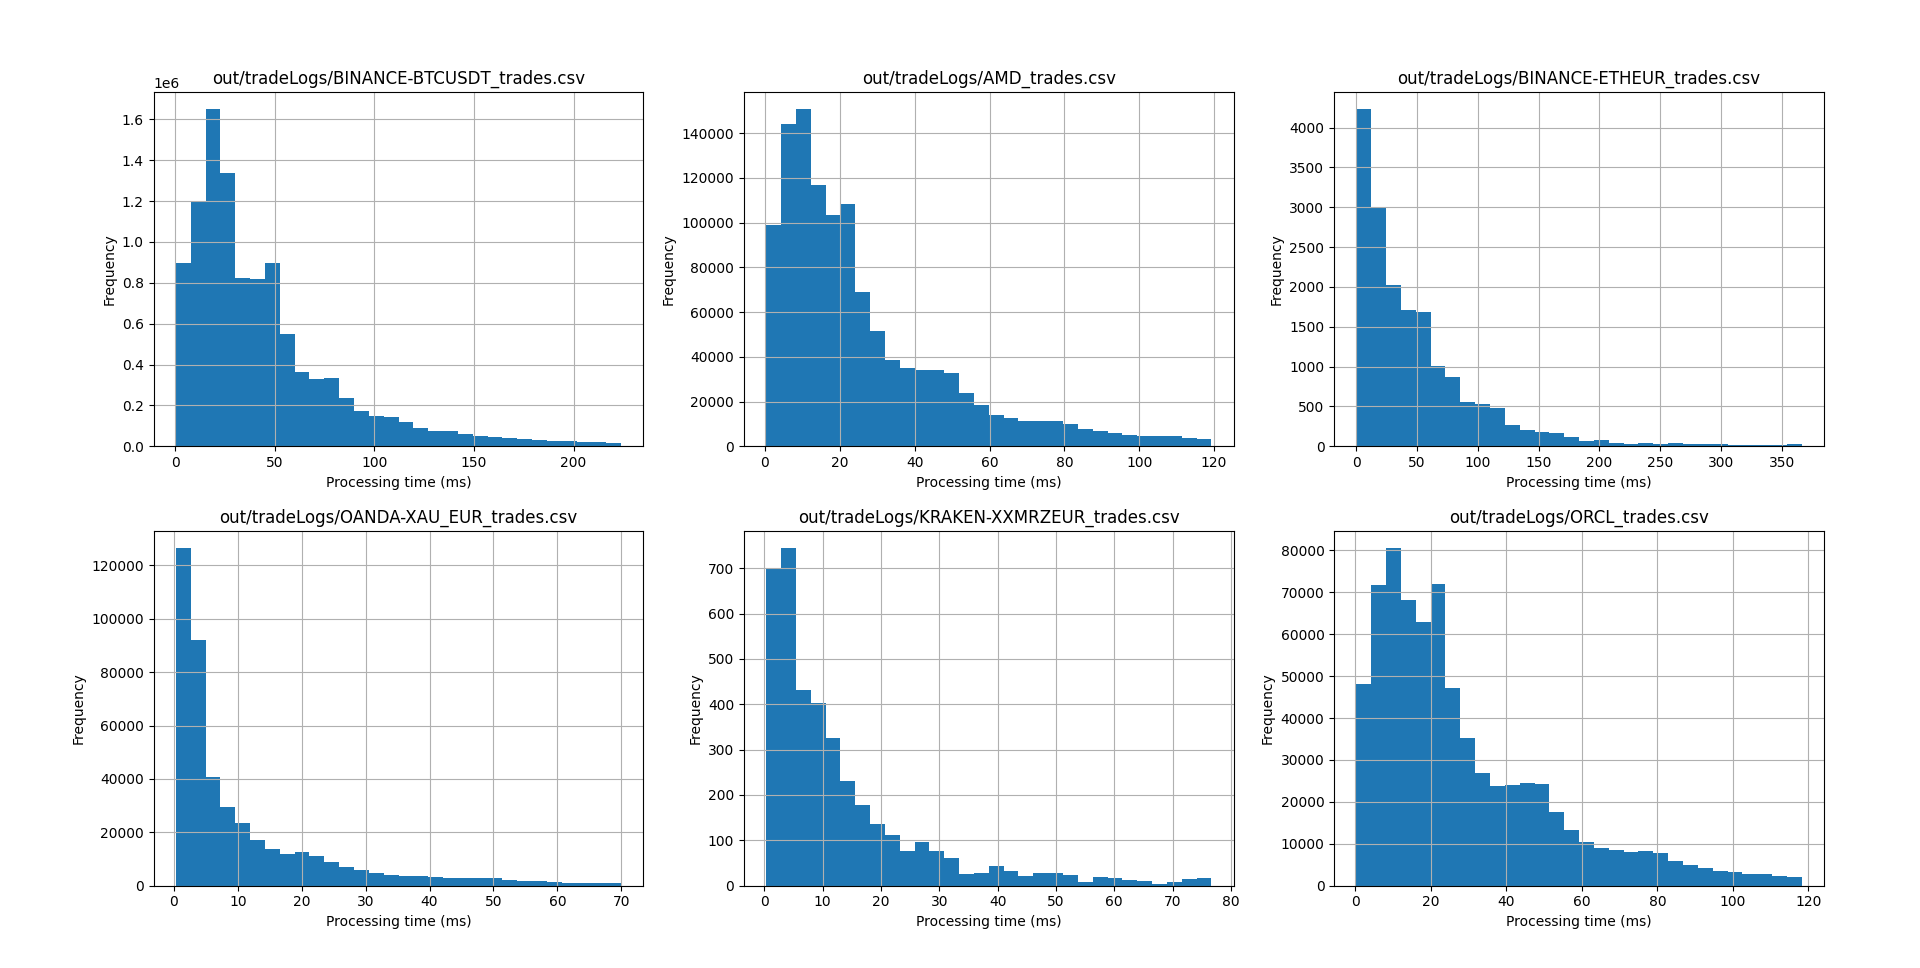
\includegraphics[width=0.95\linewidth]{./images/histogram-per-symbol.png}
\captionof{figure}{\label{fig:histogram-per-symbol}Ιστογράμματα χρόνου επεξεργασίας ανά σύμβολο}
\end{center}

\begin{center}
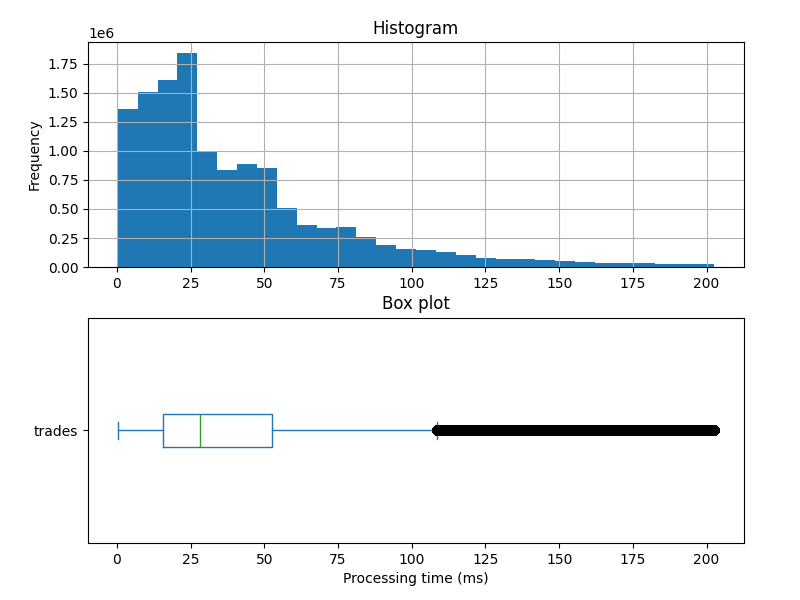
\includegraphics[width=0.5\linewidth]{./images/histogram-boxplot.png}
\captionof{figure}{\label{fig:histogram-boxplot}Ιστογράμμα και θηκόγραμμα του χρόνου επεξεργασίας όλων των συμβόλων}
\end{center}
\subsubsection{Πόροι συστήματος}
\label{sec:org95a568c}
\begin{center}
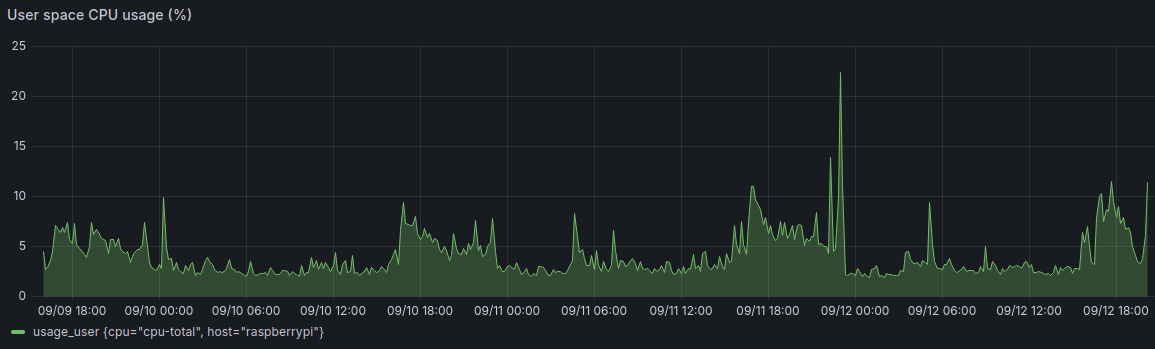
\includegraphics[width=0.7\linewidth]{./images/cpu-usage.png}
\captionof{figure}{\label{fig:cpu}Συνολικό ποσοστό χρήσης του επεξεργαστή από το user space κατά την εκτέλεση}
\end{center}

\begin{center}
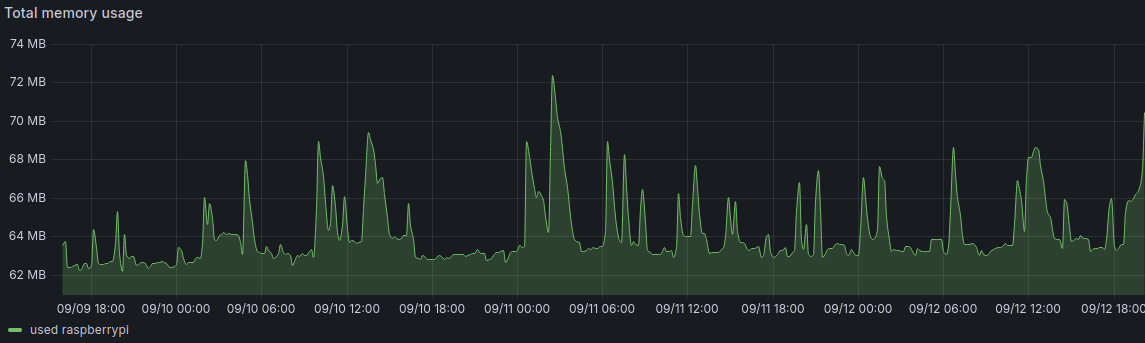
\includegraphics[width=0.7\linewidth]{./images/memory-usage.png}
\captionof{figure}{\label{fig:mem}Συνολική χρήση μνήμης κατά την εκτέλεση}
\end{center}
\subsection{Παρατηρήσεις}
\label{sec:org58a605c}
Σύμφωνα με τα διαγράμματα \ref{fig:histogram-per-symbol} και \ref{fig:histogram-boxplot}, ο χρόνος επεξεργασίας των συναλλαγών ακολουθεί γεωμετρική κατανομή, όπως ήταν αναμενόμενο. Επιπλέον, από το θηκόγραμμα του σχήματος \ref{fig:histogram-boxplot}, φαίνεται πως έχουμε πολλά πιθανά outliers, το οποίο εξηγείται από την συμπεριφορά του τρόπου αποθήκευσης των δεδομένων από το λειτουργικό σύστημα (ΛΣ), αλλά και απο την φύση της κατανομής. Για παράδειγμα, η αποθήκευση των δεδομένων μπορεί να καθυστερήσει πολύ όταν το ΛΣ δίνει προτεραιότητα σε εγγραφές άλλων προγραμμάτων. Ακόμη, η καθυστέρηση αυτή εξηγείται από την ταχύτητα αποθήκευσης των δεδομένων στην κάρτα SD ή αν την δεδομένη χρονική στιγμή που θέλουμε να εγγράψουμε η κάρτα είναι απασχολημένη για οποιοδήποτε άλλον, άγνωστο για εμάς, λόγο. Τέλος, η μέση καθυστέρηση θα ήταν αρκετά χαμηλότερη τα δεδομένα αποθηκευόταν σε έναν σκληρό δίσκο, είτε μηχανικό είτε SSD.

\printbibliography[heading=bibnumbered]
\end{document}
